\documentclass[main.tex]{subfiles}
\begin{document}
\newpage
\section{Дополнения}\label{appendix}

\begin{figure}[H]
	\centering
	\begin{subfigure}{.5\textwidth}
		\centering
		\includegraphics[width=\linewidth]{all/tsne/2d}
		\captionsetup{width=.8\linewidth}
		\caption{нефильтнованные данные на плоскости}
		\label{fig:all_tsne_2d}
	\end{subfigure}%
	\begin{subfigure}{.5\textwidth}
		\centering
		\includegraphics[width=\linewidth]{all/tsne/3d}
		\captionsetup{width=.8\linewidth}
		\caption{нефильтрованные данные в трёх измерениях}
		\label{fig:all_tsne_3d}
	\end{subfigure}

	\begin{subfigure}{.5\textwidth}
		\centering
		\includegraphics[width=\linewidth]{significant/tsne/2d}
		\captionsetup{width=.8\linewidth}
		\caption{данные с учётом только значимых полиморфизмов (на плоскости)}
		\label{fig:signif_tsne_2d}
	\end{subfigure}%
	\begin{subfigure}{.5\textwidth}
		\centering
		\includegraphics[width=\linewidth]{significant/tsne/3d}
		\captionsetup{width=.8\linewidth}
		\caption{данные только с учётом значимых полиморфизмов (в трёх измерениях)}
		\label{fig:signif_tsne_3d}
	\end{subfigure}
	\caption{Результат сокращения размерности с помощью t-SNE}
\end{figure}

\begin{figure}[H]
    \centering
    \begin{subfigure}{.5\textwidth}
        \centering
        \includegraphics[width=\linewidth]{significant/manhattan/heatmap}
        \captionsetup{width=.8\linewidth}
        \caption{расстояние Хэмминга (Манхэттенская метрика)}
        \label{fig:heatmap_manh}
    \end{subfigure}%
    \begin{subfigure}{.5\textwidth}
        \centering
        \includegraphics[width=\linewidth]{significant/impact/heatmap}
        \captionsetup{width=.8\linewidth}
        \caption{расстояние с учётом значимости}
        \label{fig:heatmap_impact}
    \end{subfigure}

    \begin{subfigure}{.5\textwidth}
        \centering
        \includegraphics[width=\linewidth]{significant/allele/heatmap}
        \captionsetup{width=.8\linewidth}
        \caption{расстояние с учётом аллельности}
        \label{fig:heatmap_allele}
    \end{subfigure}%
    \begin{subfigure}{.5\textwidth}
        \centering
        \includegraphics[width=\linewidth]{significant/impact_allele/heatmap}
        \captionsetup{width=.8\linewidth}
        \caption{расстояние с учётом значимости и аллельности}
        \label{fig:heatmap_impact_allele}
    \end{subfigure}
    \caption{Тепловые карты, построенные по матрицам расстояний (учтены только полиморфизмы с аннотациями)}
\end{figure}

\begin{figure}[H]
    \centering
    \begin{subfigure}{.5\textwidth}
        \centering
        \includegraphics[width=\linewidth]{significant/manhattan/nj}
        \captionsetup{width=.8\linewidth}
        \caption{расстояние Хэмминга (Манхэттенская метрика)}
        \label{fig:nj_manh}
    \end{subfigure}%
    \begin{subfigure}{.5\textwidth}
        \centering
        \includegraphics[width=\linewidth]{significant/impact/nj}
        \captionsetup{width=.8\linewidth}
        \caption{расстояние с учётом значимости}
        \label{fig:nj_impact}
    \end{subfigure}

    \begin{subfigure}{.5\textwidth}
        \centering
        \includegraphics[width=\linewidth]{significant/allele/nj}
        \captionsetup{width=.8\linewidth}
        \caption{расстояние с учётом аллельности}
        \label{fig:nj_allele}
    \end{subfigure}%
    \begin{subfigure}{.5\textwidth}
        \centering
        \includegraphics[width=\linewidth]{significant/impact_allele/nj}
        \captionsetup{width=.8\linewidth}
        \caption{расстояние с учётом значимости и аллельности}
        \label{fig:nj_impact_allele}
    \end{subfigure}
    \caption{Деревья, построенные метдом объединения соседей по матрицам расстояний (учтены только полиморфизмы с аннотациями)}
\end{figure}

\begin{figure}[H]
    \centering
    \begin{subfigure}{.5\textwidth}
        \centering
        \includegraphics[width=\linewidth]{significant/manhattan/dm_histogram}
        \captionsetup{width=.8\linewidth}
        \caption{расстояние Хэмминга (Ман\-хэт\-тенская метрика)}
        \label{fig:hist_manh}
    \end{subfigure}%
    \begin{subfigure}{.5\textwidth}
        \centering
        \includegraphics[width=\linewidth]{significant/impact/dm_histogram}
        \captionsetup{width=.8\linewidth}
        \caption{расстояние с учётом значимости}
        \label{fig:hist_impact}
    \end{subfigure}

    \begin{subfigure}{.5\textwidth}
        \centering
        \includegraphics[width=\linewidth]{significant/allele/dm_histogram}
        \captionsetup{width=.8\linewidth}
        \caption{расстояние с учётом аллельности}
        \label{fig:hist_allele}
    \end{subfigure}%
    \begin{subfigure}{.5\textwidth}
        \centering
        \includegraphics[width=\linewidth]{significant/impact_allele/dm_histogram}
        \captionsetup{width=.8\linewidth}
        \caption{расстояние с учётом значимости и аллельности}
        \label{fig:hist_impact_allele}
    \end{subfigure}
    \caption{Распределение значений элементов в матрицах расстояний (учтены только полиморфизмы с аннотациями)}
\end{figure}

\begin{figure}[H]
    \centering 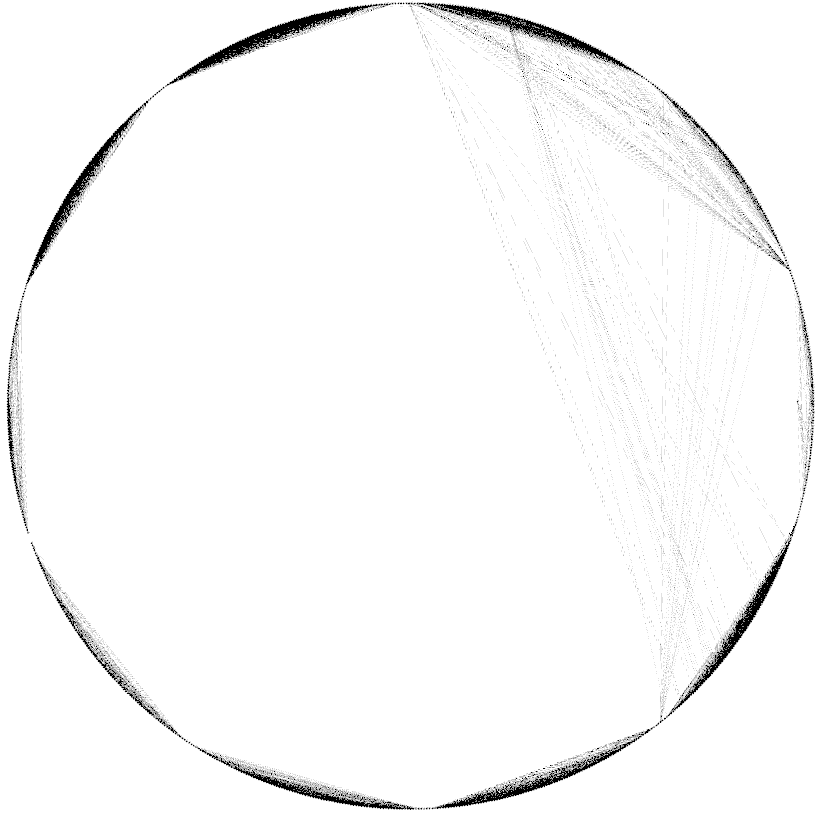
\includegraphics[width=\myPictWidth]{significant/manhattan/graph}
    \caption{Граф, построенный по матрице смежности (расстояние Хэмминга)}
    \label{fig:signif_manhattan_graph}
\end{figure}


\end{document}
